
\section{Multi-channel counter/timer}

The OpenTTP reference platform uses an Opal Kelly XEM6001 FPGA (Xilinx Spartan 6 LX16) development board to provide a multi-channel counter.
The counter is clocked at 200 MHz, so the full-range resolution is 5 ns. 
This is adequate for the applications envisaged for the OpenTTP system.

Although the counter has six channels, only three (FIXME four?) are connected in the current design \ref{f:counter}.
They are all configured with the system reference as START, with the exception of Channel 5.
This is configured with the externally input 1 pps as START, and the time-transfer receiver's 1 pps as STOP.
This is to allow time-transfer for an external reference.

The XEM6001 has eight LEDS which may aid in fault-finding \ref{t:XEM6001LEDs}. In particular, the presence of 1 pps signals 
can be readily seen (the pulses are extended so that they are visible) and the lock state of the PLL producing the 200 MHz clock.

\begin{figure}
\centerline{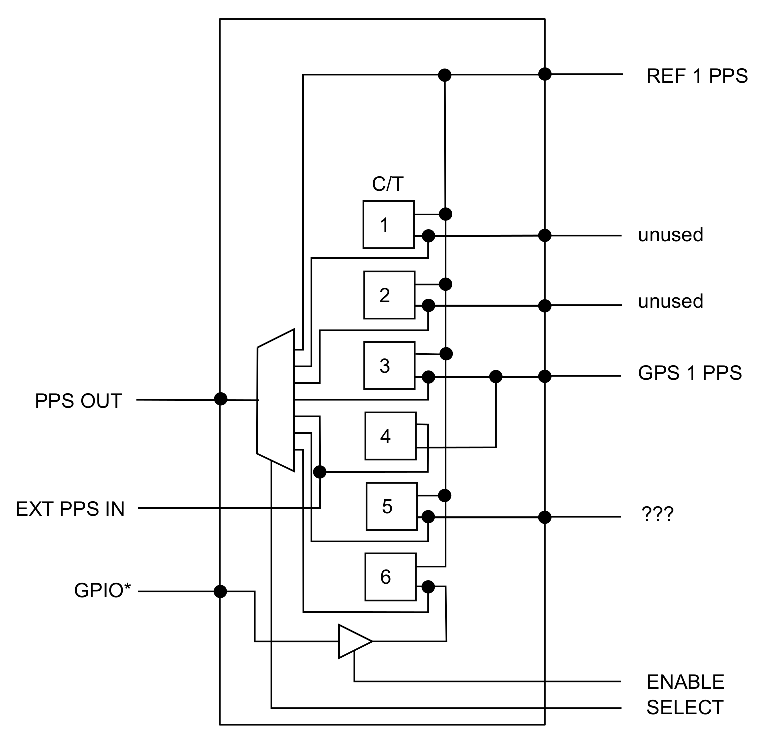
\includegraphics{figures/ottpcounter.eps}}
\caption{The OpenTTP multi-channel counter. \label{f:counter}}
\end{figure}

\begin{table}
\begin{center}
\begin{tabular}{ll}
LED & function \\ \hline
1 & channel 1 pps (unused)\\
2 & channel 2 pps (unused) \\
3 & channel 3 pps (GPS receiver)\\
4 & channel 4 pps (external pps)\\
5 & channel 5 pps (unused)\\
6 & channel 6 pps (GPIO)\\
7 & GPIO enabled\\
8 & Digital Clock Manager PLL is locked\\
\end{tabular}
\end{center}
\caption{Status LEDs on Opal Kelly XEM6001 board \label{t:XEM6001LEDs}}
\end{table}

\subsection{Counter delays}